%%%%%%%%%%%%%%%%%%%%%%%%%%%%%%%%%%%%%%%%%%%%%%%%%%%%%%%%%%%%%%%%%%%%%%%%
%                                                                      %
%     File: Inverter.tex		                                       %
%     Tex Master: Thesis.tex                                           %
%                                                                      %
%     Author: Israel Sother                                            %
%     Last modified: 27 May 2024                                       %
%                                                                      %
%%%%%%%%%%%%%%%%%%%%%%%%%%%%%%%%%%%%%%%%%%%%%%%%%%%%%%%%%%%%%%%%%%%%%%%%

\vfill
\section{Two Level Voltage Source Inverter}
\label{section:Two Level Voltage Source Inverter}%chktex 24
The usual hardware used to control synchronous machines is a 2-level Voltage Source Inverter. Such equipment is composed of six switches organized in three legs, where each pair of switches is connected to a motor terminal, as shown in \Cref{fig:inverter_and_motor_schematic}.

\begin{figure}[!htb]
	\centering
	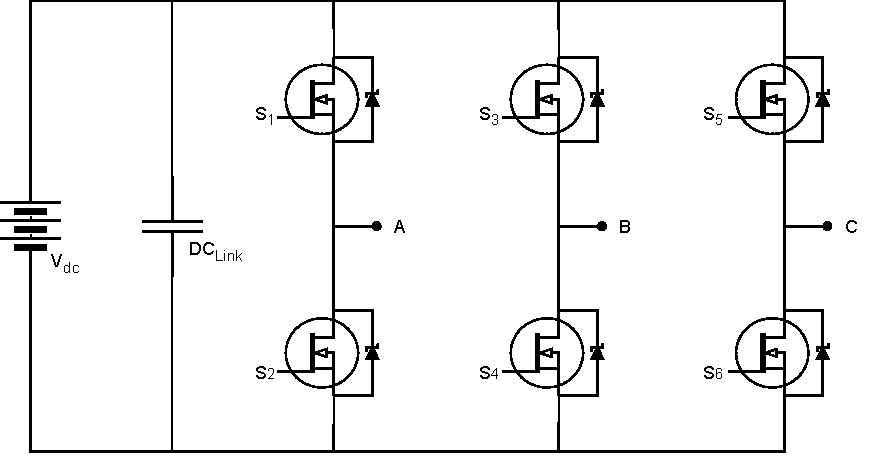
\includegraphics[width=0.7\textwidth]{Figures/Inverter.pdf}
	\caption[2-Level Voltage source Inverter arrangement.]{2-Level Voltage source Inverter arrangement.}
	\label{fig:inverter_and_motor_schematic}%chktex 24
\end{figure}

Usually, each switch in an inverter leg is operated with the inverse logic of the other switch in the leg, and this arrangement allows for 8 different switching combinations where 2 of them result in null voltages. That gives 7 possible voltage vectors, as detailed in \Cref{table:space_vector} and \Cref{fig:space_vector}. In \Cref{table:space_vector} the Vector column denotes the top switches states ($S_1$,$S_2$, and $S_3$), where a 1 means the top switch is the conducting state with the bottom switch is on a cut-off state and a 0 the opposite. The $\alpha$ and $\beta$ components which define the state space vectors are as defined by the Concordia transformation, shown in \Cref{eq:concordia}.

\begin{equation}
	\mathbf{Co} = \sqrt{\frac{2}{3}}
	\begin{bmatrix}
		1            & 0                   & \frac{1}{\sqrt{2}} \\
		-\frac{1}{2} & \frac{\sqrt{3}}{2}  & \frac{1}{\sqrt{2}} \\
		-\frac{1}{2} & -\frac{\sqrt{3}}{2} & \frac{1}{\sqrt{2}} \\
	\end{bmatrix}
	\label{eq:concordia}
\end{equation}

\begin{table}[h]
	\centering
	\caption{Switching combinations and space vectors for a 2-level three-phase inverter}
	\label{table:space_vector}%chktex 24
	\renewcommand{\arraystretch}{1.7} % more space between rows
	\resizebox{0.5\textwidth}{!}{%
		\begin{tabular}{|
				>{\columncolor[HTML]{E0E0E0}}c |
				>{\columncolor[HTML]{E0E0E0}}c |c|c|c|c|c|}
			\hline %chktex 44
			\cellcolor[HTML]{A0A0A0}\textbf{Switch State} &
			\cellcolor[HTML]{A0A0A0}\textbf{Vector}       &
			\cellcolor[HTML]{A0A0A0}\textbf{$V_{AB}$}     &
			\cellcolor[HTML]{A0A0A0}\textbf{$V_{BC}$}     &
			\cellcolor[HTML]{A0A0A0}\textbf{$V_{CA}$}	  &
			\cellcolor[HTML]{A0A0A0}\textbf{$V_{\alpha}$} &
			\cellcolor[HTML]{A0A0A0}\textbf{$V_{\beta}$}  \\ \hline %chktex 44
			0 & 000 & 0         & 0         & 0         & $0$                         & $0$                       \\ \hline %chktex 44
			1 & 001 & $V_{DC}$  & 0         & $-V_{DC}$ & $\sqrt{\frac{2}{3}}V_{DC}$  & $0$                       \\ \hline %chktex 44
			2 & 010 & $-V_{DC}$ & $V_{DC}$  & 0         & $\frac{1}{\sqrt{6}}V_{DC}$  & $\frac{1}{\sqrt{2}}V_{DC}$\\ \hline %chktex 44
			3 & 011 & 0         & $V_{DC}$  & $-V_{DC}$ & $-\frac{1}{\sqrt{6}}V_{DC}$ & $\frac{1}{\sqrt{2}}V_{DC}$\\ \hline %chktex 44
			4 & 100 & 0         & $-V_{DC}$ & $V_{DC}$  & $-\sqrt{\frac{2}{3}}V_{DC}$ & $0$                       \\ \hline %chktex 44
			5 & 101 & $V_{DC}$  & $-V_{DC}$ & 0         & $-\frac{1}{\sqrt{6}}V_{DC}$ & $\frac{1}{\sqrt{2}}V_{DC}$\\ \hline %chktex 44
			6 & 110 & $-V_{DC}$ & 0         & $V_{DC}$  & $\frac{1}{\sqrt{6}}V_{DC}$  & $\frac{1}{\sqrt{2}}V_{DC}$\\ \hline %chktex 44
			7 & 111 & 0         & 0         & 0         & $0$                         & $0$                       \\ \hline %chktex 44
		\end{tabular}%
	}
\end{table}


Despite the number of discrete voltage states, using some modulation techniques it is possible to synthesize a resultant vector if it is inside the attainable region denoted by the hexagon in \Cref{fig:space_vector}.

The current inverter used by \gls{fst} uses this structure, but the switches are silicon \glspl{igbt}, which when compared to \gls{sic} \glspl{mosfet} has a higher switching loss, leading to lower switching frequencies being used~\cite{Gurpinar:si_sic_gan_comparison:2016:IEEE}. The lower switching frequencies cause higher distortions in the current waveforms, decreasing motor efficiency. The lower switching frequency system also needs a higher capacitance on the DC Link, while the lower efficiency of silicon semiconductors requires a bigger heatsink, leading to a higher volume and mass inverter, decreasing the power density of the solution.

\subsection{Space Vector Modulation}
\label{subsection:Space Vector Modulation}%chktex 24

Several modulation techniques have been proposed in the literature like \gls{spwm}, \gls{she}~\cite{Asadzadeh:selective_harmonic_elimination:2019}, \gls{svm}~\cite{Neacsu:SVM_intro:2001:IECON}.
% , or \gls{svc}~\cite{An:space_vector_control:2016}. Some of these techniques are exclusive of multilevel inverters, like \gls{svc}~\cite{Rodriguez:svc_multilevel:2002}, while others also work for two-level inverters. 
The most common method of modulation in digital motor control is \gls{svm}, as it is a robust, easy-to-implement technique, and allows higher voltage ratio. 

% The figure "fig:space_vector" provides a visual representation of the space vector for a 2-level three-phase inverter. It shows the possible voltage states that can be applied to the motor. The phase voltages are represented in a 2D plane, with the maximum phase voltage shown by a circle. Any point within this circle is attainable without overmodulation or neutral point shift. The hexagon represents the maximum voltage that can be applied to the motor, and the vectors within the hexagon are the possible voltage states.
\Cref{fig:space_vector} shows a 2D representation of the space vector for a 2-level three-phase inverter. The basic voltage vectors (previously defined on \Cref{table:space_vector}) are shown pointing to the hexagon corners. 
% Note that they can only reach those voltages if modulation techniques that produce shifting in the neutral point (like third harmonic injection) are used.
 Connecting the basic vectors produces the hexagon of possible voltage states.

\begin{figure}[!htb]
	\centering
	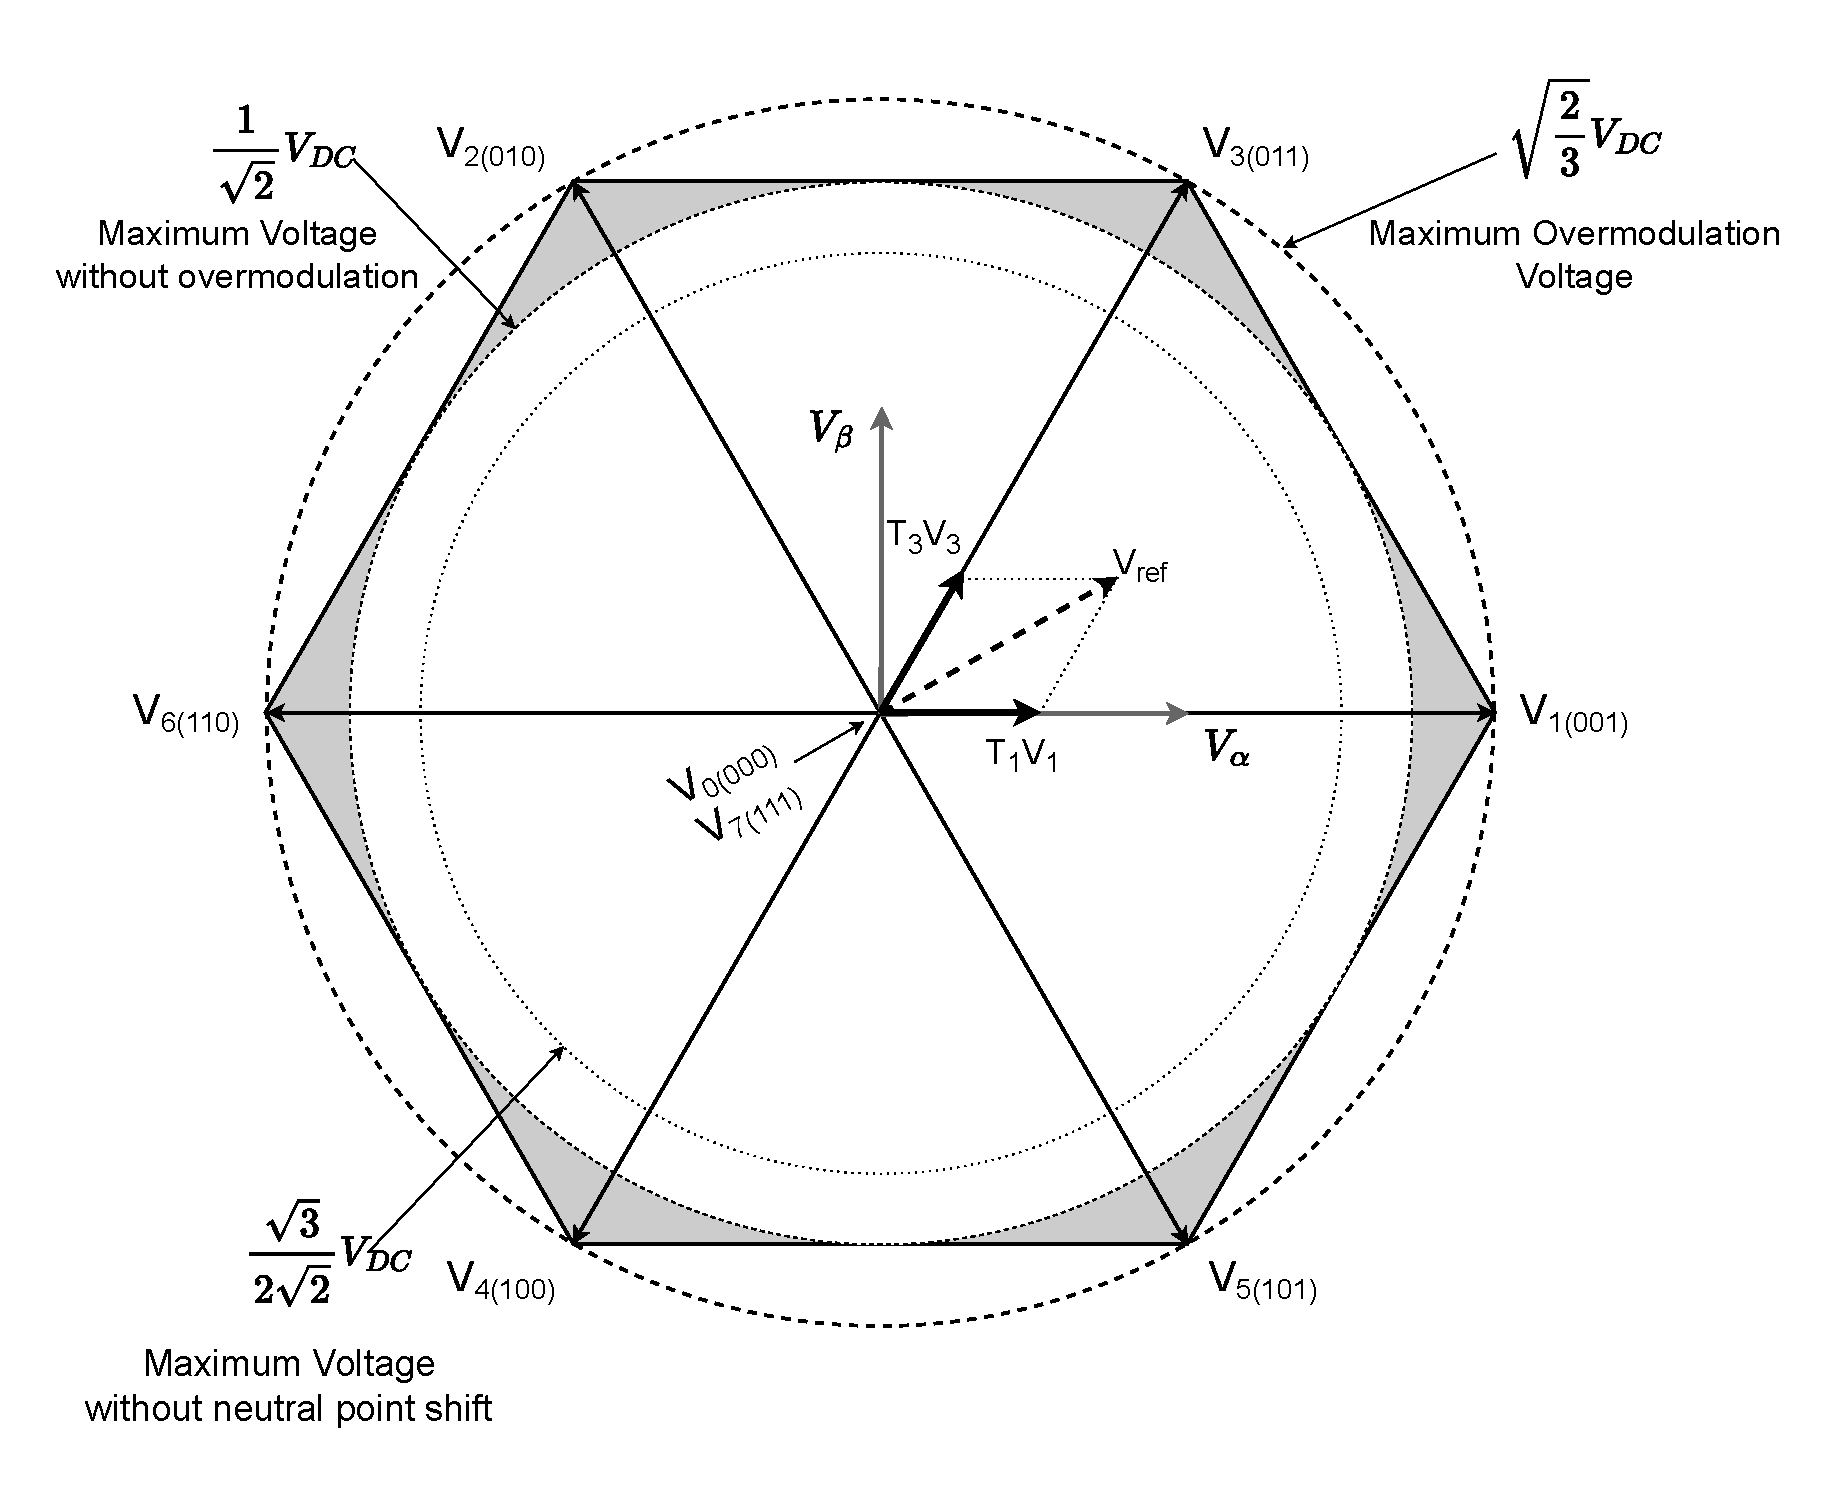
\includegraphics[width=0.8\textwidth]{Figures/Space_Vector_revised.pdf}
	\caption[Space vector for a 2-level three-phase inverter.]{Space vector for a 2-level three-phase inverter.}
	\label{fig:space_vector}%chktex 24
\end{figure}


Using \gls{svm} it is possible to modulate any vector inside the hexagon shown in \Cref{fig:space_vector}, but if a pure sinusoidal output is desired, the vectors should be constrained to the inscribed circle, that has a radius of $\frac{1}{\sqrt{2}} V_{DC}$. The reason behind this is to keep the reference vector locus inside the hexagon, avoiding distortions in the output. Note that although it is possible to generate waveforms with higher RMS value, it is not possible to modulate a peak higher than $\frac{1}{\sqrt{2}} V_{DC}$ for every vector angle. If a higher RMS value is requested the generated voltage will be saturated on the sides of the hexagon while near the corners it will achieve the requested value, thus those waveforms become more and more distorted as the amplitude approaches $\sqrt{\frac{2}{3}} V_{DC}$. To modulate a sinusoidal output the vector should develop a circular trajectory, but in the overmodulation region the voltage constrains it to the voltage hexagon, and thus the difference between the intended and the effectively applied vector increases.

To simplify the analysis of those vectors, a modulation index ($m$) is defined as shown in \Cref{eq:modulation_index}. The output is free of distortion if $m\le\frac{2}{\sqrt{3}}$, and increasing the modulation index further will result in diminishing returns in wave amplitude, while the output approaches a six-step commutation, greatly increasing the \gls{thd}~\cite{Microchip:Overmodulation:2023}. This area of operation is called overmodulation, and several approaches have been proposed~\cite{Briz:overmodulation_technique_field_weakening:2001,MehriziSani:advanced_modulation_techniques:2007} to minimize the distortions.
\begin{equation}
	m = \frac{2\sqrt{2}}{\sqrt{3}}\frac{\left|V{ref}\right|}{V_{DC}} \quad \quad m \;\in\; \left[0, \frac{4}{3}\right]
	\label{eq:modulation_index}
\end{equation}

To modulate a voltage vector that is not exactly one of the basic voltage vectors a modulation technique is needed. When using the \gls{svm} method to compose a given reference vector $V_{ref}$, the algorithm first detects the sector on which the reference vector lays. With the sector identified a ratio between the adjacent basic vectors and a null vector is selected so that the average vector is equal to the reference vector. This ratio is calculated as shown in \Cref{eq:svm_vref}.

For example, let's consider the reference vector shown in \Cref{fig:space_vector}. According to \gls{svm}, this vector can be modulated by using $V_1$ for half of the active time and $V_3$ for the other half of the active time. The active time refers to the duration when the vector amplitude is non-zero, while the null time refers to the duration when a null vector is used to reduce the output amplitude. This modulation can be expressed by \Cref{eq:svm_vref}, where $t_1+t_3$ represents the active time and $t_{n}$ represents the null time.

\begin{equation}
	V_{ref} = \frac{t_{n} V_{n} + t_1 V_1  + t_3 V_3}{h}
	\label{eq:svm_vref}
\end{equation}

%% epxplanation of the neutral point shift. it should follow the following equation: V_shift = K_{shift}*max(V_{AN},V_{BN},V_{CN) + (1-K_{shift})*min(V_{AN},V_{BN},V_{CN)


In the hardware implementation, the voltage reference is generated in the rotor reference frame (dq0) and then the inverse dq0 transformation is applied to obtain the phase voltages directly, without selecting a sector to know which vectors to use. These phase voltages are then divided by the DC link voltage to obtain the duty cycle of the switches. Note that this does not account though for the neutral point shift. This simplification results in the same switching times for the active vectors as the geometric approach of calculating which sector the reference vector is and then decomposing the reference vector in the two adjacent vectors. The null vector distribution between $V_0$ and $V_7$ will dictate the neutral point shifting method.

Several approaches have been proposed to accomplish this shift and they all rely on injecting a variable offset voltage on the neutral point that has a strong third harmonic component. Although a pure third harmonic sine wave can be used it is computationally expensive when compared with other methods such as top, mid, or bottom clamp. This technique of mid-clamp aims to center the neutral point between the DC link terminals, while the top clamp shifts the neutral point to the maximum voltage and the bottom clamp to the minimum voltage. The main advantage of a top or bottom clamp is the reduced number of switching events when compared with a mid-clamp. 

The chosen approach is defined by \Cref{eq:neutral_point_shift}, where $K_{shift}$ is the shift factor, and $V_{AN}$,$V_{BN}$, and $V_{CN}$ are the phase voltages referenced to a virtual neutral point that is the average of the phase voltages with respect to the DC link negative terminal. The value of $K_{shift}$ dictates the shift method used, when it is equal to 1 the top-clamp method is used, if it is 0.5 then the mid-clamp is used, and 0 results in the bottom-clamp method.~\citet{Microchip:ZSM_viewer:2023} has a visualization tool with the main methods shown. The calculated shift voltage is then summed to the desired phase voltages, and the modulation technique is applied as usual. In the implementation, this results in the \glspl{mosfet} duty cycle being shifted to center at the value of $K_{shift}$.

\begin{equation}
	V_{shift} = K_{shift} - K_{shift} \max \left(V_{AN},V_{BN},V_{CN}\right) - (1-K_{shift}) \min \left(V_{AN},V_{BN},V_{CN}\right)
	\label{eq:neutral_point_shift}
\end{equation}
